% Two-exchange example: line of equilibria p1 = p2 and the converging
% spread trajectories (slope -1), with the two eigen-directions.
\begin{center}
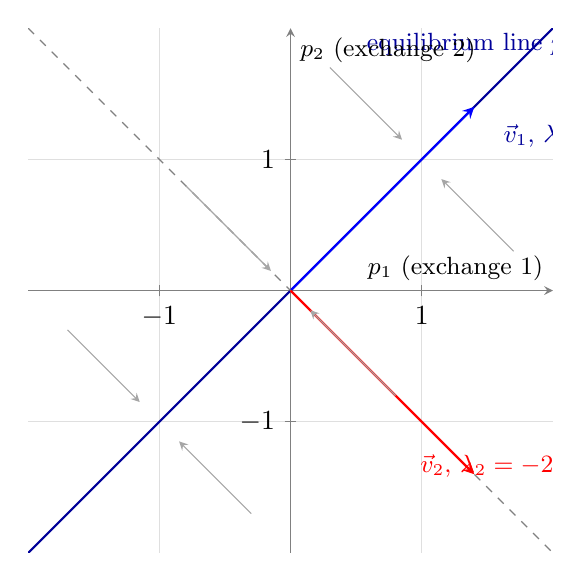
\begin{tikzpicture}
\begin{axis}[
  width=0.68\linewidth, height=0.68\linewidth,
  xlabel={$p_1$ (exchange 1)}, ylabel={$p_2$ (exchange 2)},
  axis lines=center,
  axis line style={gray},
  label style={font=\small},
  xmin=-2, xmax=2, ymin=-2, ymax=2,
  xtick={-1,0,1}, ytick={-1,0,1},
  grid=major, grid style={gray!25},
]
% line of equilibria: p1 = p2
\addplot[domain=-2:2, thick, blue!60!black, samples=2] {x};
\node[blue!60!black, font=\small, anchor=south] at (axis cs:1.6,1.72) {equilibrium line $p_1 = p_2$};
% eigenvector v1 lies along that line (lambda1 = 0)
\draw[thick, blue, -stealth] (axis cs:0,0) -- (axis cs:1.4,1.4);
\node[blue!60!black, font=\small, anchor=west] at (axis cs:1.55,1.18) {$\vec{v}_1$, $\lambda_1 = 0$};
% spread direction: p1 + p2 = 0
\addplot[domain=-2:2, dashed, gray, samples=2] {-x};
% eigenvector v2 (lambda2 = -2k)
\draw[thick, red, -stealth] (axis cs:0,0) -- (axis cs:1.4,-1.4);
\node[red, font=\small, anchor=north] at (axis cs:1.55,-1.18) {$\vec{v}_2$, $\lambda_2 = -2k$};
% spread trajectories: slope -1, arrows toward the diagonal
\draw[gray!70, -stealth] (axis cs:0.8,-0.8)  -- (axis cs:0.15,-0.15);
\draw[gray!70, -stealth] (axis cs:-0.8,0.8)  -- (axis cs:-0.15,0.15);
\draw[gray!70, -stealth] (axis cs:1.7,0.3)   -- (axis cs:1.15,0.85);
\draw[gray!70, -stealth] (axis cs:0.3,1.7)   -- (axis cs:0.85,1.15);
\draw[gray!70, -stealth] (axis cs:-0.3,-1.7) -- (axis cs:-0.85,-1.15);
\draw[gray!70, -stealth] (axis cs:-1.7,-0.3) -- (axis cs:-1.15,-0.85);
\end{axis}
\end{tikzpicture}
\end{center}
